\section{電流帰還バイアス回路の動作点設定(直流の話)}
電流帰還バイアス回路は、エミッタ接地増幅回路の基本形であり、増幅回路の直流電流動作点を決めるための動作原理図である。(実際にこの形のままで使われることはない。)
固定バイアス、自己バイアス等、入力信号(電圧)にバイアスを加える方法はいくつかあるが、一般的に、トランジスタの持つ特性により動作に悪影響を受ける。(直流電流増幅率の温度変化)
この回路は、温度変化による影響を受けにくい設計となっている。

\begin{description}
  \setlength{\parskip}{0cm} % 段落間
  \setlength{\itemsep}{0cm} % 項目間
  \item[ゴール] 前章で決めた動作点と諸条件から直流電流の動作点を決める。(ブリーダ抵抗の値を決定する。)
  \item[キーワード] ブリーダ抵抗、温度補償
  \item[ストーリー] 前章で決めた動作点+諸条件 → 閉路方程式を立てて回路に流れる直流電流を求める。→ 直流電流の動作点を決める。→ LTspice上で設計 → DCスイープにより動作点を確認 → 計算値と比較
\end{description}

\subsection{原理・計算}
$V_{CC}$ を $R_1$ と $R_2$ で分圧することで、ベース電位 $V_{BQ}$ を設定する。
添え字 Q がバイアス計算で求める量である。\\

\begin{figure}[htbp]
  \begin{center}
  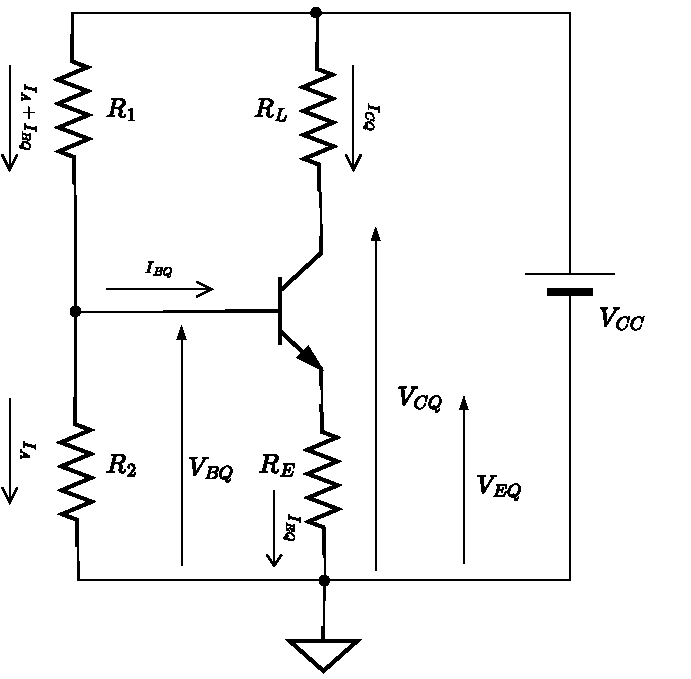
\includegraphics[width=0.45\linewidth]{img/43.pdf}
  \caption{電流帰還バイアス回路の原理図}
  \end{center}
\end{figure}


$I_{BQ} \approx 0$ と近似(他の電流と比べて小さいため)すると、$R_1$ を流れる電流は、全て$R_{2}$ に流れるので、\\
$$V_{BQ} \approx \frac{R_2}{R_1+R_2}V_{CC}$$ により、ベースのバイアス電圧が求まる。ベース電流がゼロなので、$r_b$ による電圧降下はゼロである。(ベース層の抵抗)\\
$I_{EQ} = \frac{V_{EQ}}{R_E}$ ($V_{EQ}$ は $R_E$ の両端電圧)\\
$V_{EQ} = V_{BQ} - V_{BE}$ ($V_{BE}$ は、前のシミュレーションで求めた約 0.7 V の値を使う。)\\
$I_{CQ} \approx I_{EQ} (I_{EQ} = I_{CQ} - I_{BQ} \approx 0)$\\
$V_{CQ} = V_{CC} - R_LI_{CQ}$\\
$I_{BQ} = \frac{I_{CQ}}{\beta_0}$ ($\beta_0$: 直流電流増幅率)

\subsection{回路の特徴}
\begin{enumerate}
  \setlength{\parskip}{0cm} % 段落間
  \setlength{\itemsep}{0cm} % 項目間
  \item 温度補償\\
  トランジスタの直流電流増幅率は、温度によって上昇する性質がある。
  $\beta_{0}$ 増加 → $I_{CQ}$ が増加 → $I_{EQ}$ も増加 → $R_{E}I_{EQ}$ が増加\\
  $V_{BE} = V_{BQ} - V_{CQ}$ より、$V_{BE}$ が減少 → $I_{BQ}$ が減少 → $I_{CQ}$ の増加を抑制する。
  \item 利点: 温度が変化した場合のバイアス安定度が高い。
  \item 欠点: $R_2$ を比較的小さく設定する関係で、これらの抵抗に流れる電流(ブリーダ電流)により、消費電流が大きくなる。
\end{enumerate}

\subsection{電流帰還バイアス回路の設計手順}
電流帰還バイアス回路を設計するためにあらかじめ条件が要求される。
\begin{enumerate}
  \setlength{\parskip}{0cm} % 段落間
  \setlength{\itemsep}{0cm} % 項目間
  \item 諸条件の設定
  \begin{itemize}
    \item 使用するトランジスタ:2SC1815
    \item 直流増幅率$\beta_0 = 213$
    \item $V_{BE} = 0.7386$ V
    \item $V_{CC} = 10$V
    \item バイアス点電流$I_{CO}=5.5$mA
    \item $I_{BO}= \frac{I_{CO}}{\beta_0} = \frac{5.5\times10^{-3}}{213} \approx 25.82 \mu$A
    \item $R_E$による電圧降下は、$V_{CC}$の10\verb|%| とする。
    \item $V_{CEO} = V_{RLO}$とする。
    \item ブリーダ電流$I_A$: $I_{BO}$ の20倍
  \end{itemize}
  \item $R_E$を求める\\
  $V_{EO} = R_EI_{EO} = 0.1V_{CC} = 1.0$ V $I_{EO} \approx I_{CO}$ より
$$R_E = \frac{V_{EO}}{I_{CO}} = \frac{1}{5.5 \times 10^{-3}} \approx 181.818 \Omega$$
  \item $R_L$を求める\\
  $R_L$ に流れる電流 $I_{CO}$ について、$V_{CEO} = V_{CO} -V_{EO}$ と $R_LI_{CO}$ を等しくすると、出力信号の振幅を最大化できる。(動作点を負荷線の真ん中に選ぶ)
  \item ブリーダ電流$I_A$を求める。\\
  $20 \times I_{BO} = 20 \times 25.82 \mu$ A $= 0.5164$ mA
  \item $R_2$を求める\\
  $V_{BO} = R_2I_A$ より、$$R_2 = \frac{V_{BO}}{I_A} = \frac{(V_{EO}+V_{BE})}{I_A} = \frac{(1+0.7386)}{0.5164}\textrm{mA}$$ $$\approx 3366.769946 \approx 3.4 \textrm{k}\Omega$$
  \item $R_1$を求める
  $$R_1 = \frac{(V_{CC} - (V_{EO}+V_{BE}))}{I_A+I_{BO}} = \frac{(10 - (1+0.7386))}{(0.5164 \times 10^{-3} + 25.82\mu)} = 15236.25097 \approx 15.2 \textrm{k}\Omega$$
\end{enumerate}

\subsection{LTspiceで演習}
これらの計算値を用いて回路を設計する。
\subsubsection{DC動作点解析}
\begin{description}
  \setlength{\parskip}{0cm} % 段落間
  \setlength{\itemsep}{0cm} % 項目間
  \item [課題10] 以下の回路を作成し、.opディレクティブを用いてDC動作点解析をして下さい。\\
  DC動作点が正しく設定されているかどうか考えて下さい。
  \begin{figure}[htbp]
    \begin{center}
    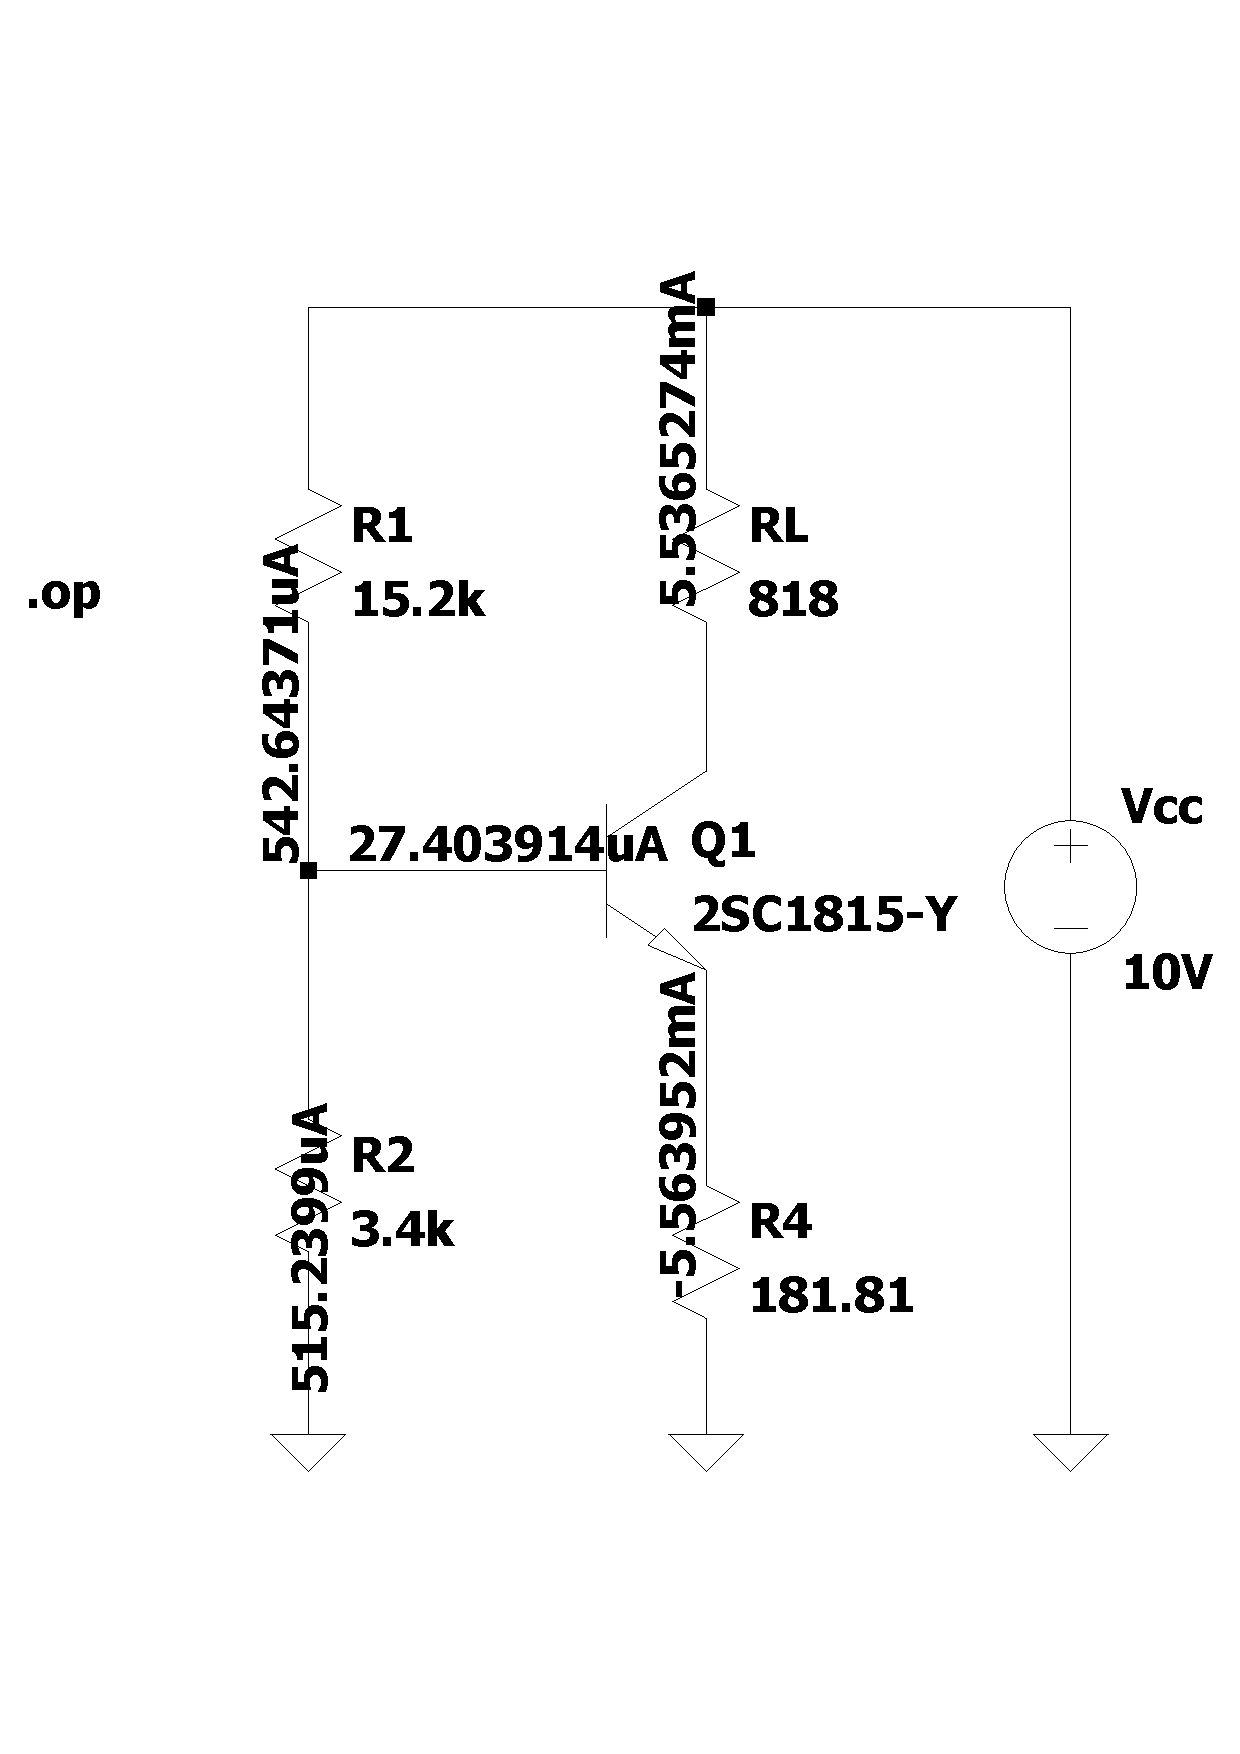
\includegraphics[width=0.4\linewidth]{img/44.pdf}
    \caption{電流帰還バイアス回路DC動作点解析}
    \end{center}
  \end{figure}
\end{description}